\section{Mask Propagation}
\label{sec:mask_propagate}

Video object segmentation is a task that requires specific objects to be segmented in a given video. In terms of Semi-supervised settings, a first-frame annotation is provided by the user, and the method segments objects in all remaining frames automatically. This technique, which uses a mask as prior knowledge to predict other masks, is called Mask Propagation.

To propagate these sparse labels through the entire video sequence, traditional methods often solve an optimization problem with an energy defined over a graph structure \cite{badrinarayanan2010label}, \cite{vijayanarasimhan2012active}, \cite{avinash2014seamseg}.

Early deep neural network methods rely on fine-tuning the networks at test time to make segmentation networks focus on target objects and then inference on all other frames, which are extremely slow. Among them, OSVOS \cite{caelles2017one} and MoNet \cite{xiao2018monet} finetune pre-trained networks on the first-frame ground-truth at test time. OnAVOS \cite{voigtlaender2017online} extends the first-frame fine-tuning by introducing an online adaptation mechanism. Following these approaches, MaskTrack \cite{perazzi2017learning} and PReM \cite{luiten2018premvos} utilize optical flow to help propagate the segmentation mask from one frame to the next. Despite achieving promising results, the test-time fine-tuning restricts networks’ efficiency. 
Faster approaches have been proposed such as temporal CNN, capsule routing \cite{duarte2019capsulevos}, tracking, space-time matching, and memory-based methods:

\textbf{Temporal CNN}. Recurrent methods propagate information often from the most recent frames, either via a mask \cite{perazzi2017learning} or via a hidden representation \cite{ventura2019rvos}, \cite{hu2017maskrnn}. These methods are prone to drifting and struggle with occlusions.

\textbf{Tracking}
In contrast, tracking-based approaches \cite{jang2017online}, \cite{wang2019fast}, \cite{chen2020state} perform
frame-to-frame propagation and are thus efficient at test-time. They however lack long-term context and often lose track after object occlusions.

\textbf{Space-time matching}. While some methods \cite{huang2020fast}, \cite{voigtlaender2019feelvos} \cite{yang2020collaborative} also include the first reference frame for global matching, the context is still limited and it becomes harder to match as the video progresses

\textbf{Memory-based}. To address the context limitation, recent state-of-the-art methods use more past frames as feature memory \cite{oh2019stm}, \cite{duarte2019capsulevos}, \cite{huang2020fast} ,\cite{ge2021video}, \cite{cheng2021stcn}, \cite{cheng2022xmem}, \cite{yang2022associating}. These approaches leverage a memory network to embed past-frame predictions into memory and apply non-local attention mechanisms to propagate object information from the memory to the current frame. Our work strongly adopts the memory-based style. 

Oh et. al \cite{oh2019stm} introduces a framework which extract embeddings from multiple intermediate frames and store inside the memory. Then in forwarding stage, these memories are combined with the query embeddings to segment the object

\begin{figure}[!h]
    \centering
    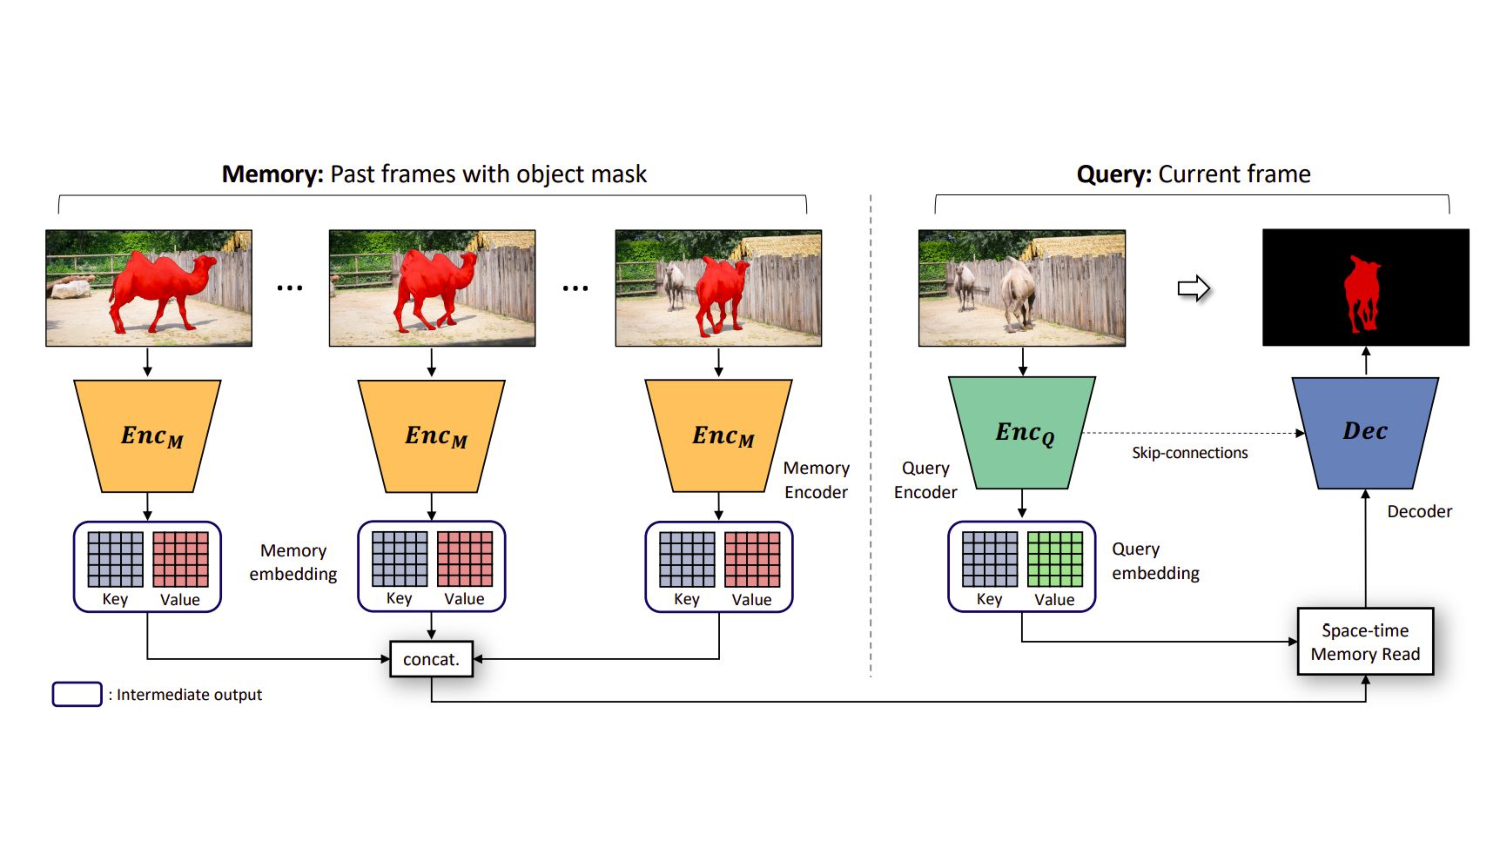
\includegraphics[width=\textwidth]{content/resources/new_images/models/stm.pdf}
    \caption{Overview architecture of STM \cite{oh2019stm}.}
    \label{fig:stm}
\end{figure}

Cheng et. al  \cite{cheng2021mivos} proposes a framework in which the user initially scribbles a mask of an object, the scribble is transformed into the real binary mask (S2M), then that mask is propagated through every video frame based on STM \cite{oh2019stm}. Then the user can choose some incorrect frames and scribble to guide the fusion with the propagated frame to output more accurate masks (Different-aware fusion).

\begin{figure}[!h]
    \centering
    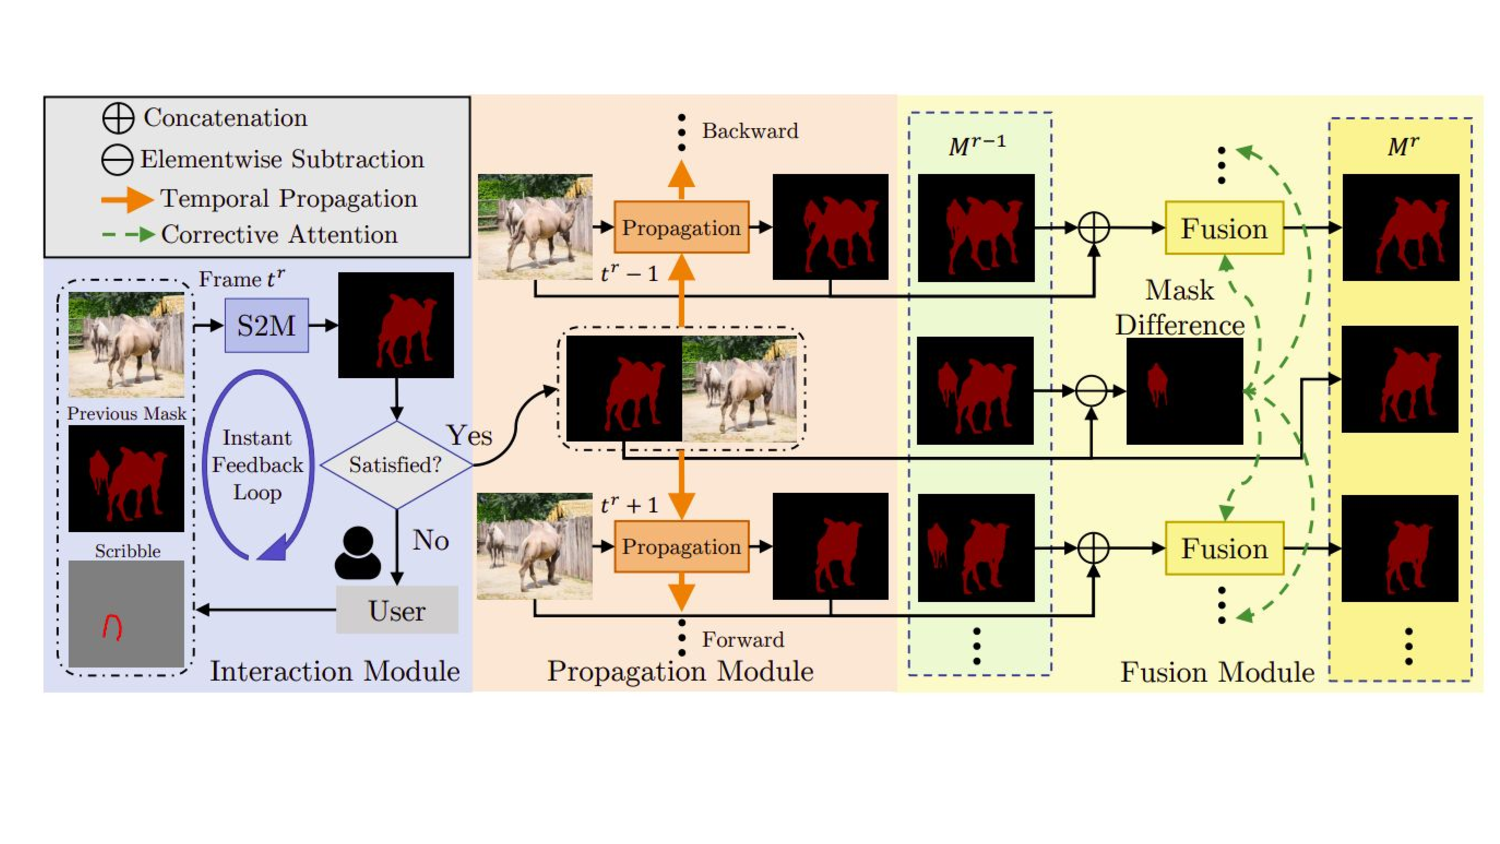
\includegraphics[width=\textwidth]{content/resources/new_images/models/mivos.pdf}
    \caption{Overview architecture of MiVOS \cite{cheng2021mivos}}
    \label{fig:mivos}
\end{figure}

Among these extensions, we adapt STCN \cite{cheng2021stcn} as one of our main modules for refinement as it is simple and effective. but with minor modification. However, most variants cannot handle long videos due to the ever-expanding feature memory bank of STM.

\begin{figure}[!h]
    \centering
    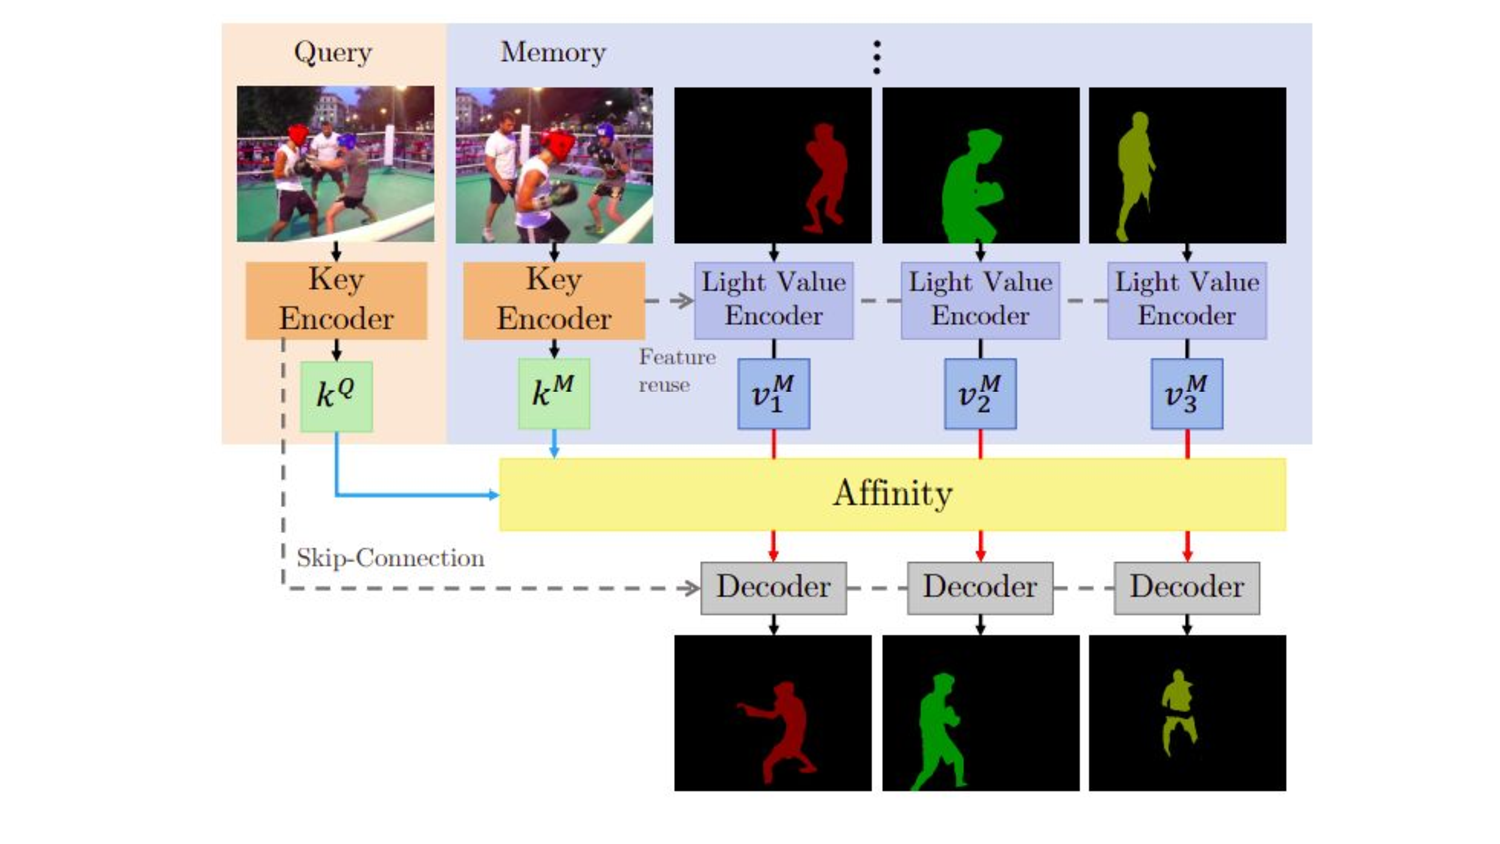
\includegraphics[width=\textwidth]{content/resources/new_images/models/stcn.pdf}
    \caption{Overview architecture of STCN \cite{cheng2021stcn}}
    \label{fig:stcn}
\end{figure}

Nonetheless, the mask propagation and segmentation are still computed individually for different objects. The
problem restricts the application and development of the VOS with multiple targets. Hence,  \cite{yang2022associating} proposes AOT to associate and decode multiple targets simultaneously, as efficiently as processing a single object. Moreover, it is the first method to utilize Transformer modules inside mask-propagation

\begin{figure}[!h]
    \centering
    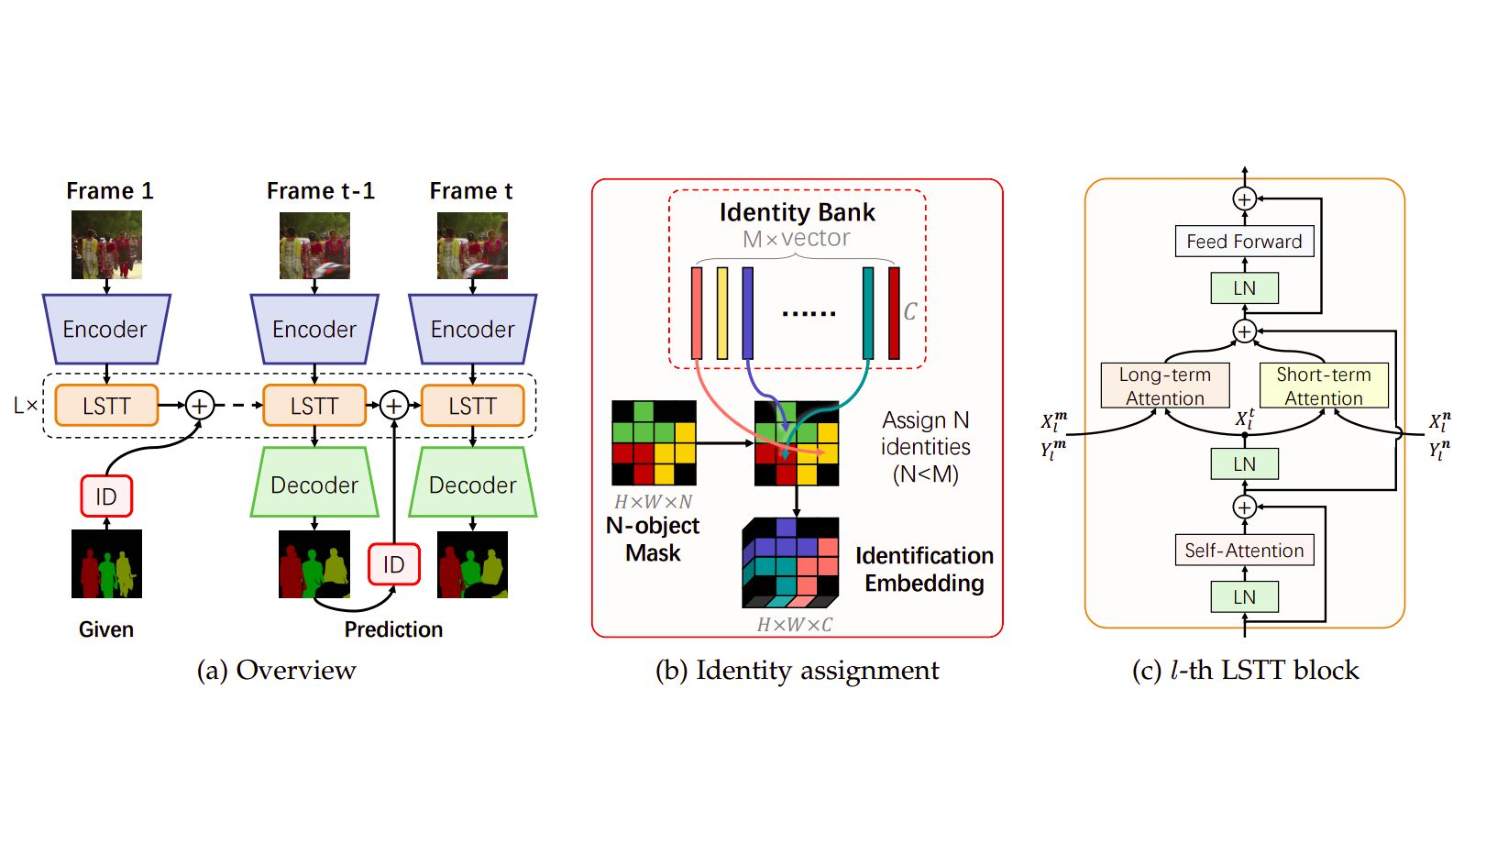
\includegraphics[width=\textwidth]{content/resources/new_images/models/aot.pdf}
    \caption{Overview architecture of AOT \cite{yang2022associating}}
    \label{fig:aot}
\end{figure}

Yet, it still does not solve the GPU memory explosion problem. Recently, authors of STCN \cite{cheng2021stcn}, develop XMem \cite{cheng2022xmem} which uses multiple memory stores to capture different temporal contexts while keeping the GPU memory     usage strictly bounded due to the long-term memory and consolidation.

\begin{figure}[!h]
    \centering
    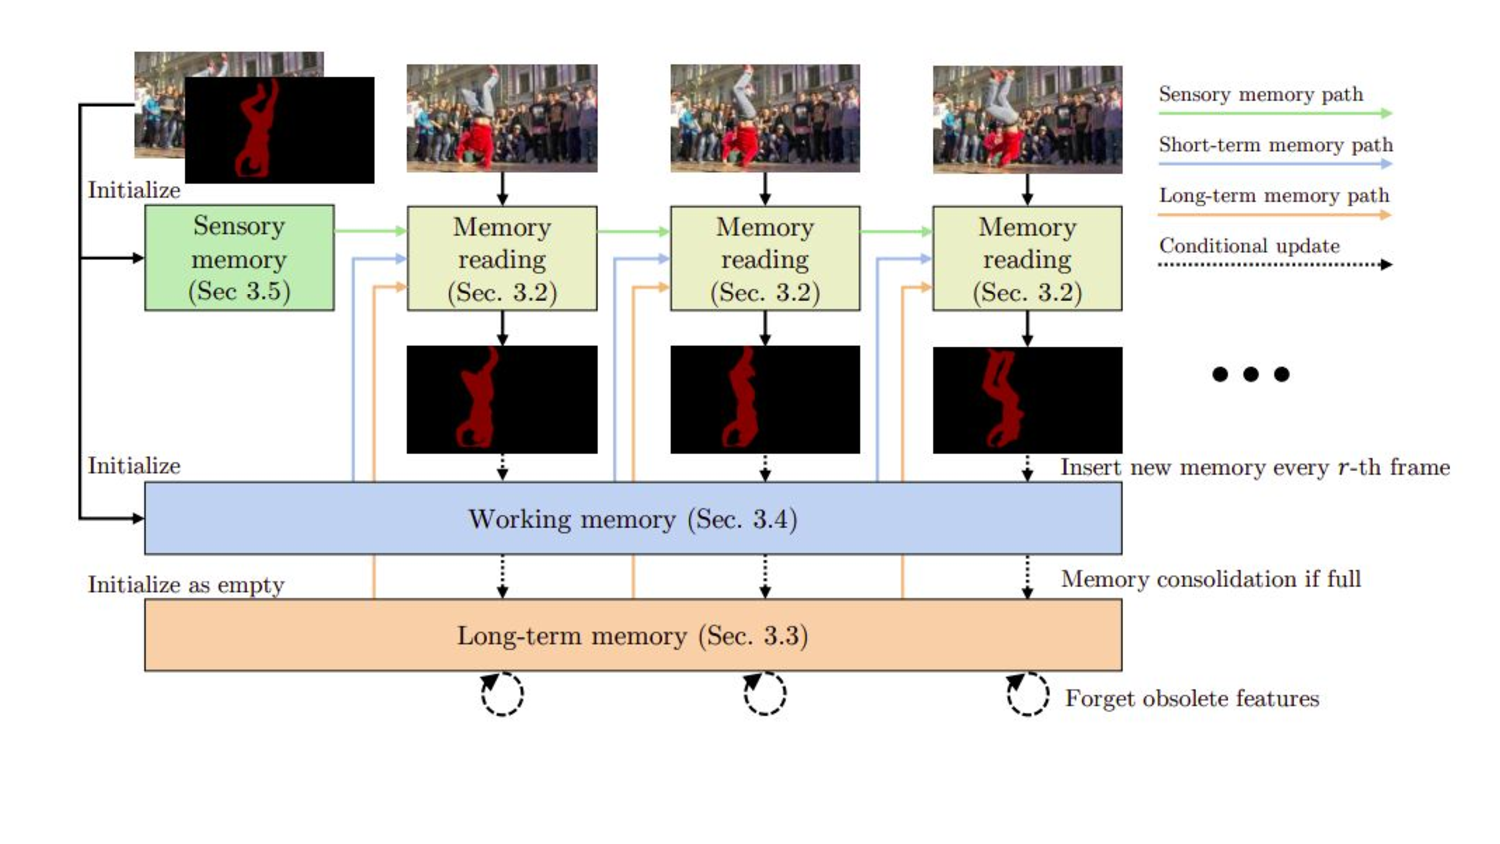
\includegraphics[width=\textwidth]{content/resources/new_images/models/xmem.pdf}
    \caption{Overview architecture of XMem \cite{cheng2022xmem}}
    \label{fig:xmem}
\end{figure}


Although video object segmentation has yielded promising results in a number of domains, these approaches have not been exploited for medical dataset creation. The use of medical images for training and testing machine learning algorithms is critical to the development of accurate models that can be used to diagnose and treat diseases. In order to improve the accuracy and effectiveness of machine learning algorithms for medical image analysis, it is important to develop novel methods specifically tailored for this domain. Mask propagation is a popular technique in interactive scenarios of video object segmentation. 

The user will refine the inputs to the algorithm in order to segment the target objects more accurately. Our proposed concept is heavily inspired by the DAVIS Challenge on Video Object Segmentation. After the first raw prediction of the associate model, the user will interact with some of the valuable slices. After that, they will submit their predicted masks to a server for review. In each of these subsequent interactions, from a list of slices specified by themselves, they choose one frame with an uncertain prediction and provide it to a server who then provides them with a new set of scribbles in this frame which points out regions that are false positives or negatives 



